\documentclass[12pt]{article}

\usepackage{float, graphicx}
\usepackage[margin=2.5cm]{geometry}
\usepackage{amsmath, amsthm, amssymb}
\usepackage{wrapfig}
\usepackage[lined,boxed,commentsnumbered]{ algorithm2e }
\graphicspath{ { ./img/ } }
\newtheorem{definition}{Definition}

\usepackage{setspace}
\doublespacing

\begin{document}

\begin{titlepage}
	\begin{center}
		~\\[2.5cm]
		{\Huge Simulating Detachment of Tumor Cell Clusters}\\[1.5cm]
		{\Large HGEN 396: Human Genetics Research Project}\\[7.0cm]
		\emph{Student:}\\
		Mr. Zafarali Ahmed (260560472)\\[1.0cm]
		\emph{Supervisor:}\\
		Dr. Simon Gravel\\[1.0cm]
		\emph{Submission Date:}\\
		\today\\[1.0cm]
		\emph{Location:}\\
		McGill University
	\end{center}
\end{titlepage}

\begin{abstract}
Blood of patients with cancer contain Circulating Tumor Cells (CTCs). Recent advances in capture technology find that CTCs exist in single cells as well as clusters \cite{Aceto2014}. Studies have hypothesized their relative contributions to metastasis, including the controversial role of plakoglobin. We implement the Cellular Potts Model to simulate the detachment of a tumor cell from a tumor. This paper works to test the feasability of such a model and if it can be used to make theoretical predictions.
\end{abstract}

\section{Introduction}
Cancer is the autonomous and uncontrolled growth of cells that forms a feed forward system to reinforce the tumors’ existence \cite{hallmarks}. Cancer originates from accumulated mutations in tumor supressor genes, proto-onco genes and DNA repart genes. These mutations hinder the cells' abillity to regulate cell cycles and they divide uncontrollably. However, for cancerous cells to keep growing and overcome the limitations due to diffusion of nutrients, tumors have two solutions: angiogenesis and metastasis. While angiogenesis permits tumors to grow blood vessels and bring in nutrients, metastasis is the migration of cancer cells to other parts of the body often via the blood vessels. It is often after metastasis that cancer becomes difficult to contain and treat despite surgical resection \cite{Hatzikirou2012}.

For the tumor cells to perform invasion, the first step in metastasis, the migrating cell must alter cell surface interaction with its microenvironment: neighboring cells and the extra cellular matrix. Altered expression of cell adhesion molecules like cadherins, catenins and plakgoblin facilitate these changes in interactions \cite{Aktary2012}. Once in the blood stream, they are referred to as Circulating Tumor Cells (CTCs).

In a recent study \cite{Aceto2014}, CTC-Chip and CTC-iChip isolation of blood from patients with breast cancer verified the existence of both Single-CTCs and CTC-Clusters. Despite being rare, these clusters demonstrated (i) higher metastatic potential, (ii) faster disease progression and were found to (iii) originate directly from the tumor rather than aggregate in the blood.

Capturing the above tumor dynamics, we attempt to use the Cellular Potts Model to simulate and investigate parameters resulting in the formation of single-CTCs and CTC-clusters.

\section{Purpose and Objectives}
Since metastasis is the \emph{point of no return} for most patients, it is necessary to build intuition of the factors that lead to the production of single-CTCs versus CTC-clusters and the sizes of CTC-clusters produced. Since CTC-clusters have elevated metastatic potential and lethality, understanding how they detach from the parent tumors can lead to possible therapeutic strategies.

Our objective with this paper is to build and test the feasibility of a toy model that can easily be extended to account for the formation for single-CTCs and CTC-clusters. This toy model can eventually be used to make theoretical predictions.

\section{Materials and Methods}
\subsection{Cellular Potts Model (CPM)}
The Cellular Potts Model \cite{Graner1992} is a simple, yet powerful, model was used to simulate tissue cultures.  The model is an extension of the q-Potts Model in statistical mechanics. It consists of a $M\times M$ lattice of \emph{spins}. For a more biological interpretation, we can consider a \emph{spin} to represent an area of \emph{cell cytoplasm}. At any location of the lattice $(x,y)$, a spin can take on a value $\sigma(x,y) = \{0,1,\cdot N\}$. A \emph{cell}, $\sigma$, is defined as a colelction of these spins; as such this restricts same-spin values to be neighbours of each other. If $\sigma(x,y) = 0$, then this region is said to be the \emph{extra cellular matrix (ECM)}. To be able to simulate different \emph{types} of cells, for example proliferating and migrating cells, we introduce $\tau(\sigma)$, which returns the \emph{type} of the cell $\sigma$. Two cells can be seen in Figure \ref{basic}.
%% @TODO figures to show comparison?!?!%

For each position on the lattice, we define a \emph{Hamiltonian} $H$, as follows:
\[
	H = H_{surface} + H_{area} + H_{gradients}
\]
\begin{itemize}
	\item $H_{surface}$ characterizes the surface tension between a cell $\sigma$ and its neighbours.
	\item $H_{area}$ captures the dynamics of cells being restricted to a certain size.
	\item $H_{gradients}$ captures any external forces applied to cells due to chemical potentials and other pertubations.
\end{itemize}

The simulation then proceeds via a Monte Carlo method to flip spins in the lattice in an attempt to grow and move cells. Cells will move to minimize this Hamiltonian.

\subsection{Hamiltonian Equations}
Cells experience surface tensions when they interact with their environment, this effect is captured by the following Hamiltonian function:

\begin{equation}
	H_{surface} (x,y) = \sum_{\sigma' \in \text{neighbours}~\sigma} J(\tau(\sigma), \tau(\sigma'))(1-\delta(\sigma, \sigma'))
\end{equation}

$J(\tau_1, \tau_2)$ is the cell-interaction function that returns the surface tension between two cell types and $\delta$ is the Kronecker delta function, $\delta(x,y)=\{1:~\text{if }x=y;~0:~\text{otherwise}\}$. The Kronecker delta function prevents us from considering two lattice positions of the same spin to have a surface tension since these two spins are part of the same cell.

Cells cannot grow indefinitely. If cells are too big they cannot efficiently diffuse nutrients and shuttle machinery within its cell boundaries. This effect can be captured by the following Hamiltonian:

\begin{equation}
	H_{area} = \sum_{\text{all spins }\sigma} (a_{current}(\sigma)-a_{target})^2 \cdot \theta(a_{target}(\sigma))
\end{equation}

Here $a_{current}(\sigma)$ and $a_{target}(\sigma)$ are functions that return the current and target area of the cell respectively, and $\theta(x)=\{0:~\text{if}~x\leq 0; 1:~\text{if}~x>0\}$. Here $\theta(x)$ works to prevent us from considering negative target areas. This is essential because we have defined $a_{target}(\sigma_{ECM}) < 0$.

Finally, we would like to add perturbations to our model. For example, we would like there to be an oxygen gradient towards a blood vessel that makes it energetically favorable for cells to move away from the main tissue. This effect can be captured with the following Hamiltonian:
\begin{equation}
	H_{gradients}(x,y) = V(x,y)
\end{equation}
Where $V(x,y)$ is some potential which we can change to simulate a variety of different effects.

\subsection{Monte Carlo Metropolis Algorithm}
Each \emph{spin copy attempt} of our simulation follows the algorithm outlined below \cite{Glazier2007}:

\begin{enumerate}
  \item Choose a lattice site at random $(x,y)$ with a spin $\sigma_{select}$
  \item Pick a trial spin $\sigma_{trial}$ from the neighbors of $(x,y)$
  \item Calculate $H_{initial}$ using $\sigma_{select}$
  \item Calculate $H_{final}$ using $\sigma_{trial}$
  \item Calcualte energy change, $\Delta H = H_{final} - H_{intial}$
  \item{ Change $\sigma_{select}$ to that of $\sigma_{trial}$ with the probability:
  \[
 		P(\text{Spin Copy Attempt Successful}) =
  	\begin{cases}
   		1 & \text{if } \Delta H \leq 0 \\
   		\exp{(-\frac{\Delta H}{T})}       & \text{if } \Delta H > 0
  	\end{cases}
	\]
}
\end{enumerate}

Here the temperature, $T$, accounts for thermal fluctuations and adds a stochastic element to our algorithm where a cell can change its shape to a unfavorable one if it obtains some energy from the environment in the formal of a thermal kick. The higher $T$ is, the more likely the unfavorable spin copy attempt is.

\begin{definition}[Monte Carlo Time Step (MCS)] One Monte Carlo Time Step is $M$ spin copy attempts, where $M$ is the size of the lattice.
\end{definition}

\subsection{Implementation and Parameters}
The model is implemented in the Python programming language and graphics are generated using Matplotlib\cite{matplotlib}. The parameters for all simulations are mentioned.

Performance characteristics were measured on an Apple MacBook Pro (mid-2013) running Mac OS X Yosemite ($10.10$) with $2.5$GHz Intel Core i$5$ Processor and $4$GB of $1600$MHz RAM.

All code can be found on http://www.github.com/zafarali/hgen-396/ under \emph{Cellular Potts Model}

\subsection{Simulation and Experimental Setup}
% How were the experiments set up and methodology behind it%
\begin{definition}[$k$-CTC]
A Circulating Tumor Cell Cluster containing $k$ cells, $15>k>0$.
\end{definition}

The main focus of the project is to ensure that our model can make realistic predictions. Keeping this in mind experiments were set up to test the feasability of the model and to see if it solves trivial cases and conforms to intuition. To do this, we first determine the performance of our model to check if it completes in reasonable time frames and will allow us to run larger experiments in the future. 

To check trivial cases, we run multiple single-spin cells to determine \emph{death frequency}. We expect that $15\%$ of cells will die within the first spin copy attempt. We run this experiment for $250$MCS to give cells time to expand (parameters: $a_{target}(\sigma(1))=20$ and $J(1,1)=1, J(1,0)=5$). From this data, \emph{death frequency} is measured and we can determine if cells grow to their $a_{target}$.

$k$-CTCs for $k>0$ were subject to a constant force in a $100\times100$ lattice for $10000$MCS. The resulting end-state is used to measure \emph{velocity} of their migration and other characteristics such as \emph{splitting frequency} and \emph{survival}.

Our final experiment attempted to separate a single tissue mass into two, in the presence of forces pulling on opposite ends of the lattice.

%% RESULTS
\section{Results}
\subsection{The CPM Performs in Reasonable Time Frames}
We ran the CPM for sizes $M=\{1, \ldots , 20\}$ with $N=\text{floor}(\frac{M^2}{25})$ cells for $t=500$MCS to allow simulate the worst case scenario of using every possible lattice position (parameters: $a_{target}(\sigma(1))=25$ and $J(1,1)=1, J(1,0)=5$). We take averages over three runs using the \%timeit function available in iPython.

Running time of the simulations showed an overall increasing trend (Figure \ref{runningtime}) as $M$ is increased. A $40\times40$ lattice with $64$ cells takes an average of $57.4$ seconds. This time is reasonable because if we extrapolate this trend, for simulations of $t=10,000$MCS, our simulations will complete on the order of $10$ minutes.

\subsection{The CPM Solves Single Spin Cell Situations According to Expectations}
When running single-spin cells in a lattice for $250$MCS, we observe 48 death events ($17.6\%$). The difference between expected death events and observed death events is $2.6\%$. The extra $2.6\%$ of cells that died can be accounted for by the cells that did not die within the first \emph{spin copy attempt}. This confirms our trust in the implementation of the the model.

At the end of the simulations, surviving cells had a mean area of $\mu = 17.99$ with a variance of $\sigma^2 = 6.39$ (Figure \ref{cellareas}). This is within $a_{target}(\sigma)=20$ and we can conclude that our area constraint works as expected. 

By the design of our model, it is impossible for cells to spontaneously appear. This is our final expectation of the model.

\subsection{Comparing $k$-CTCs for $10 \geq k\geq1$} %TODO%
$k$-CTCs were set up in a $100\times100$ lattice as shown in Figure \ref{racestart}. Simulations were run for $10,000$MCS, $10$ times for each value of $k$. The results are summarized in Table \ref{racestats}. For $k>2$, Mean Velocity stabilized at $25.09\times10^-3\text{MCS}^{-1}$. For $k\leq3$, the mean velocity is lower. This can be explained by the fact that for $k\geq3$, $k$-CTCs tend to move in unison while for $k=\{1,2\}$ $k$-CTCs tend to split and move at more unpredictable directions. We plot heatmaps (Figure \ref{heatmap}) of the ending positions to confirm this reasoning. $1$ and $2$-CTCs tend to have a wider range of ending positions for their cells while $k\geq3$ tend to have simillar ending configurations.

We also observe that the highest \emph{splitting frequency} is when $k=2$. When $k>3$ we see this splitting frequency drop very sharply. This suggests that larger $k$-CTCs do not tend to split as easily as their smaller counterparts. This makes sense because in larger $k$-CTCs, an escaping cell would need to break interactions with many more cells than just $1$ other cell like in the $k=2$ case.

\subsection{Tissues Can be Induced to Split in Two}
A discontinous force (Figure \ref{forceapplied}) was applied to the lattice of $N=150$ cells as shown in Figure \ref{nebula} (Top left) in an attempt to split the mass of tissues into two. It took a total of $t=15000MCS$ for the tissues to begin splitting. The results of this experiment are summarized at increasing timesteps in Figure \ref{nebula}. It is clear that we infact can split tissues into two.

Qualitative observations reveal that, tissues split starting at the outer edges akin to pulling a piece of bubble gum. This is an important observation because it rules out the sudden appearance of the Extra Cellular Matrix within the tissue and is what is expected \emph{in vivo}.
%% DISCUSSIONS
\section{Discussion}

\subsection{Model Feasibility}
%% Is this model feasible to what we are trying to do?%

\subsection{$k$-CTC Velocity is inversely proportional to $\sqrt{W}$ }
% Simons conjecture %

\section{Conclusion}


\pagebreak
\section{Tables and Figures}

\begin{figure}[H]
	\centering
	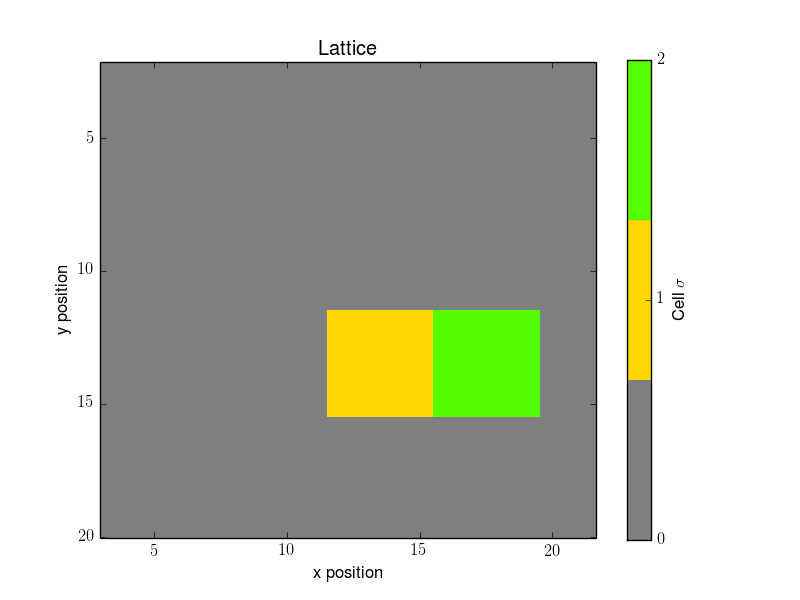
\includegraphics[scale=0.5]{img/basic}
	\caption{An example of two cells in a lattice, each color represents a different cell $\sigma$. The grey area is the Extra Cellular Matrix}
	\label{basic}
\end{figure}

\begin{figure}[H]
	\centering
	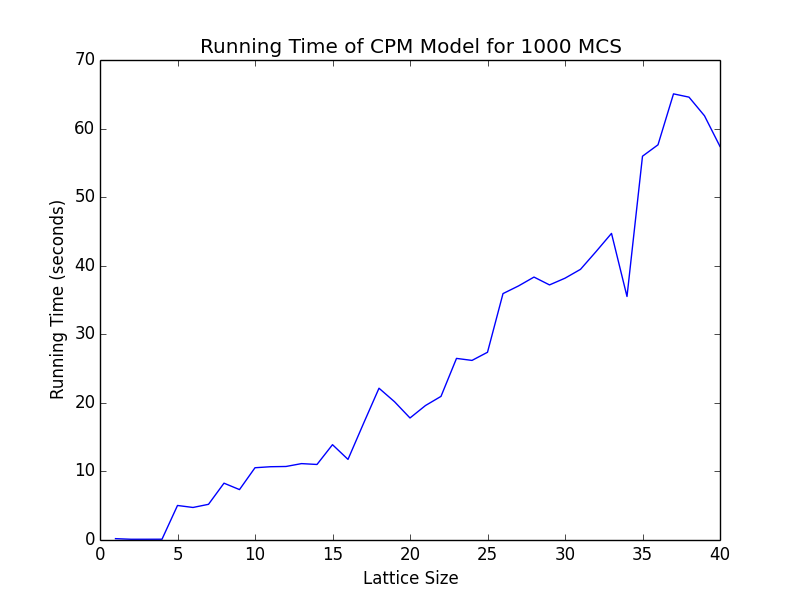
\includegraphics[scale=0.5]{img/runningtime}
	\caption{Running time for lattice size, $M =\{1,\ldots, 20\}$ and number of cells, $N=\frac{M^2}{25}$ for each simulation (average of three runs).}
	\label{runningtime}
\end{figure}

\pagebreak

\begin{figure}[H]
	\centering
	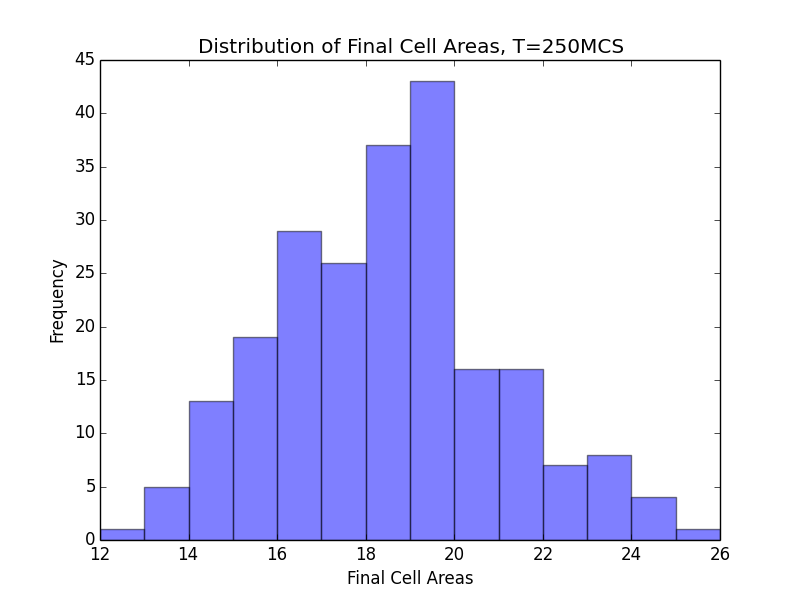
\includegraphics[scale=0.5]{img/cellareas}
	\caption{The distribution of final cell areas for $N=250$ simulations of a single-spin cell after $250$MCS. ($\mu = 17.99, \sigma^2=6.39$) }
	\label{cellareas}
\end{figure}

\begin{figure}[H]
	\centering
	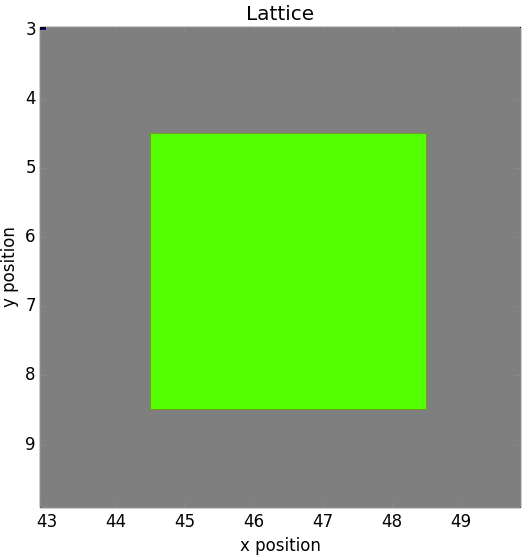
\includegraphics[scale=0.20]{img/1ctc_start}
	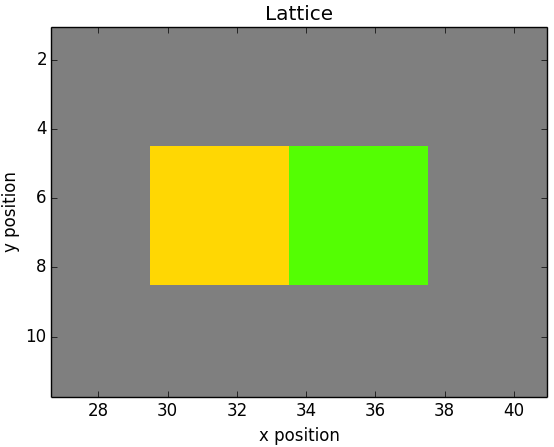
\includegraphics[scale=0.20]{img/2ctc_start}
	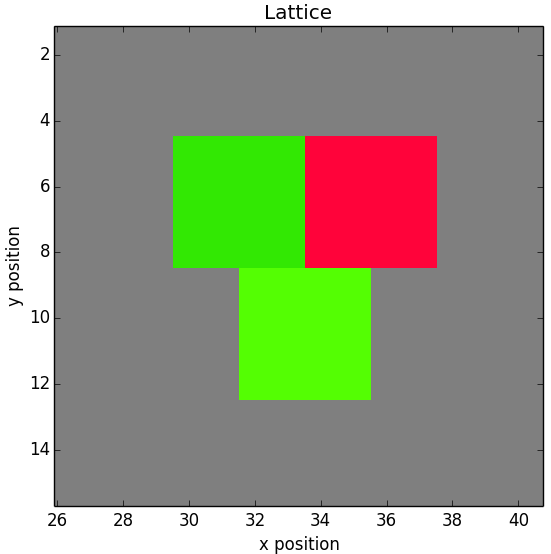
\includegraphics[scale=0.20]{img/3ctc_start}
	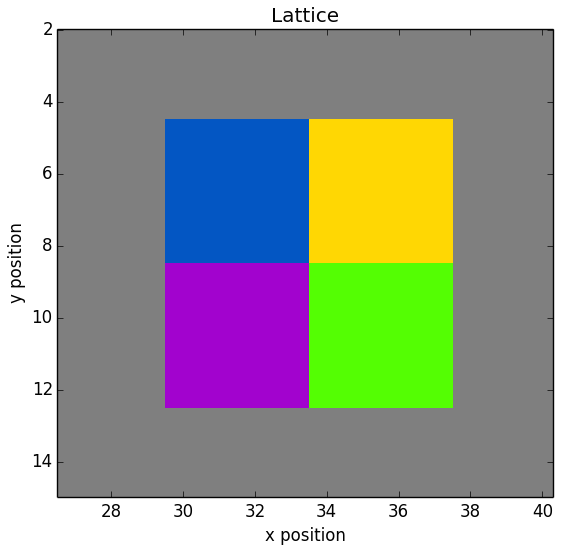
\includegraphics[scale=0.20]{img/4ctc_start}
	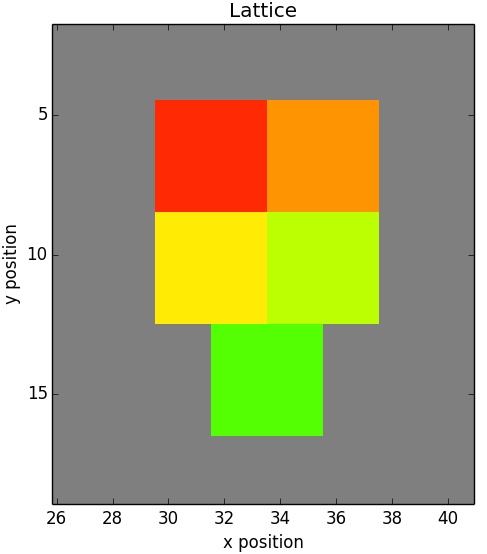
\includegraphics[scale=0.20]{img/5ctc_start}
	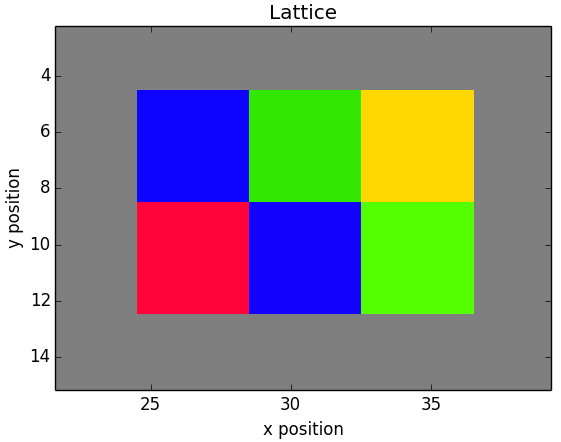
\includegraphics[scale=0.20]{img/6ctc_start}
	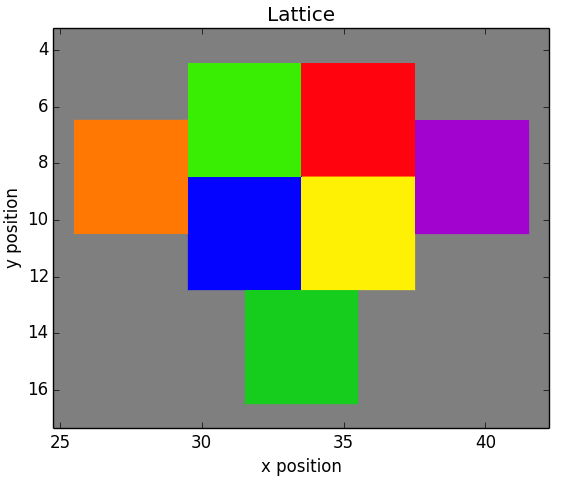
\includegraphics[scale=0.20]{img/7ctc_start}
	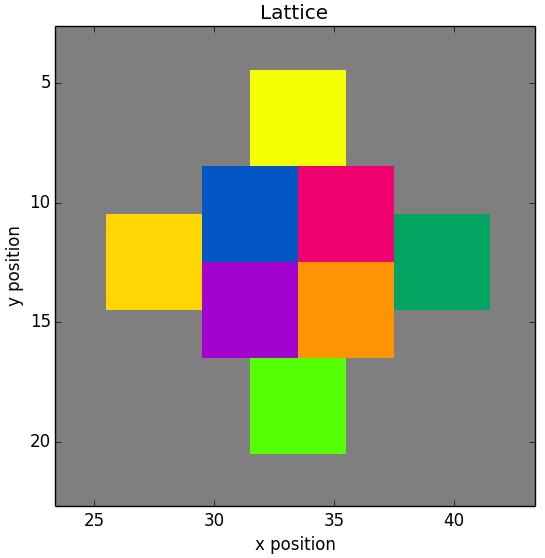
\includegraphics[scale=0.20]{img/8ctc_start}
	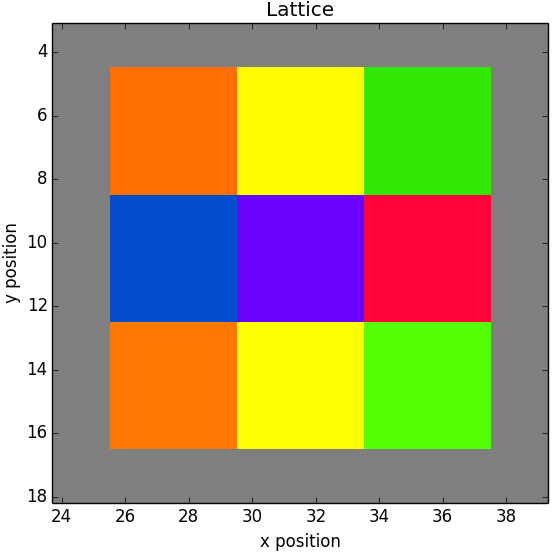
\includegraphics[scale=0.20]{img/9ctc_start}
	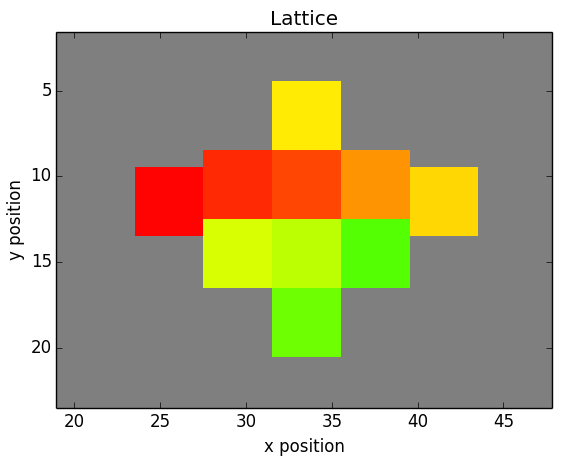
\includegraphics[scale=0.20]{img/10ctc_start}
	\caption{Starting positions of $k$-CTC for $11>k>0$.}
	\label{racestart}
\end{figure}

\begin{table}[H]
	\begin{tabular}{|l|l|l|l|l|l|l|l|l|l|l|}
	\hline
	k                                         & 1     & 2     & 3     & 4     & 5     & 6     & 7     & 8     & 9     & 10    \\ \hline
	Mean Velocity $(\frac{10^-3}{MCS})$ & 21.49 & 23.88 & 25.80 & 25.50 & 24.70 & 25.38 & 25.22 & 24.08 & 25.06 & 25.01 \\ \hline
	Variance in velocity 							& 22.89		&	7.44	&	7.24	&	0.91	&	1.47	&	0.47	&	0.72	&	1.07	&	1.07	&	1.70 \\ \hline
	Splitting Frequency              & N/A   & 0.2   & 0.06  & 0.02  & 0.03  & 0.00  & 0.01  & 0.01  & 0.02  & 0.01  \\ \hline
	Survival             & 1.00  & 1.00  & 1.00  & 1.00  & 1.00  & 1.00  & 1.00  & 1.00  & 1.00  & 1.00 \\ \hline
	\end{tabular}
	\caption{Results from running $k$-CTCs experiencing a constant force for successive $k$.}
	\label{racestats}
\end{table}
\pagebreak
\begin{figure}[H]
	\centering
	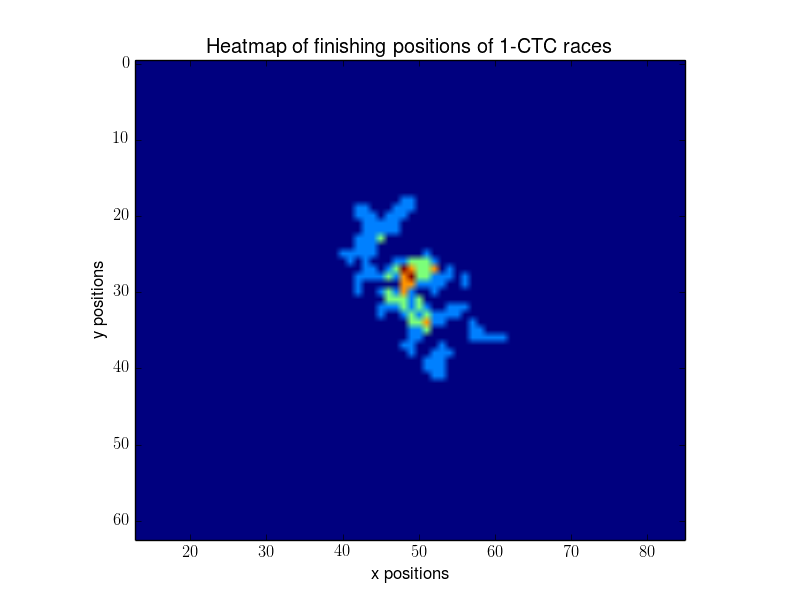
\includegraphics[scale=0.40]{img/1ctc_heat}
	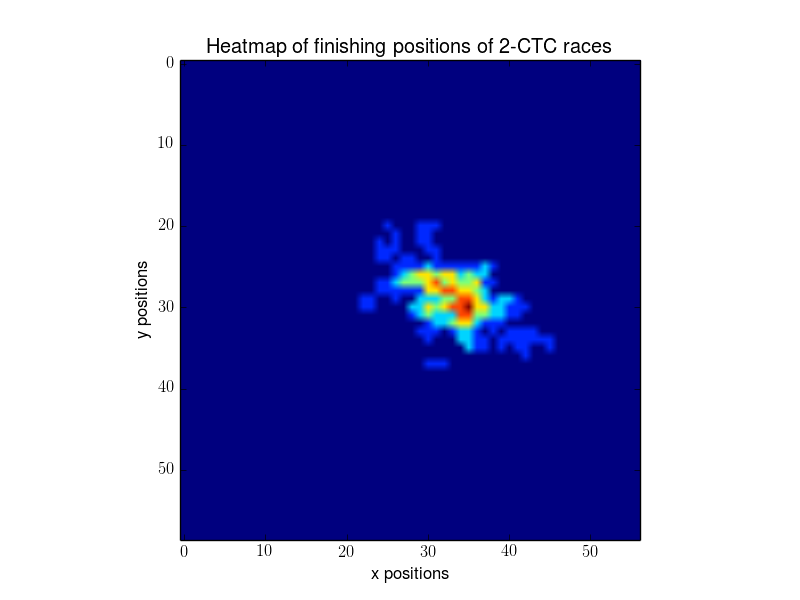
\includegraphics[scale=0.40]{img/2ctc_heat}
	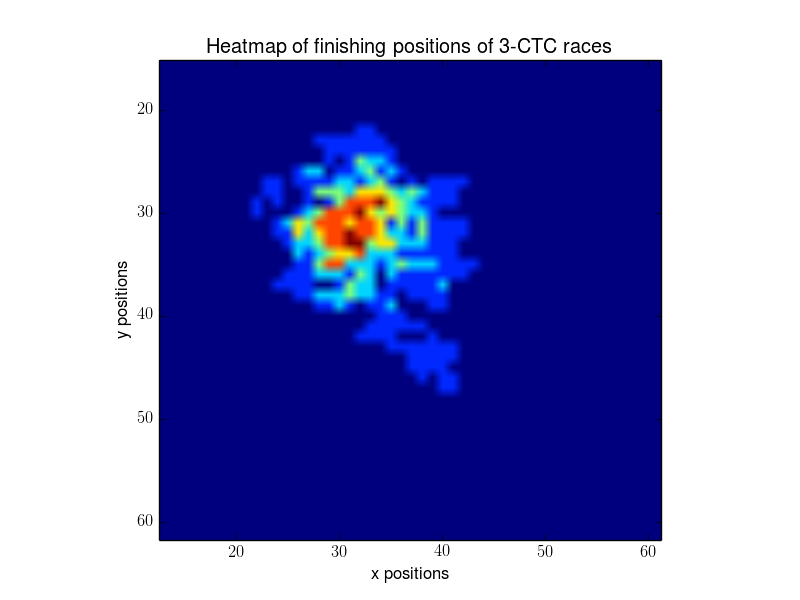
\includegraphics[scale=0.40]{img/3ctc_heat}
	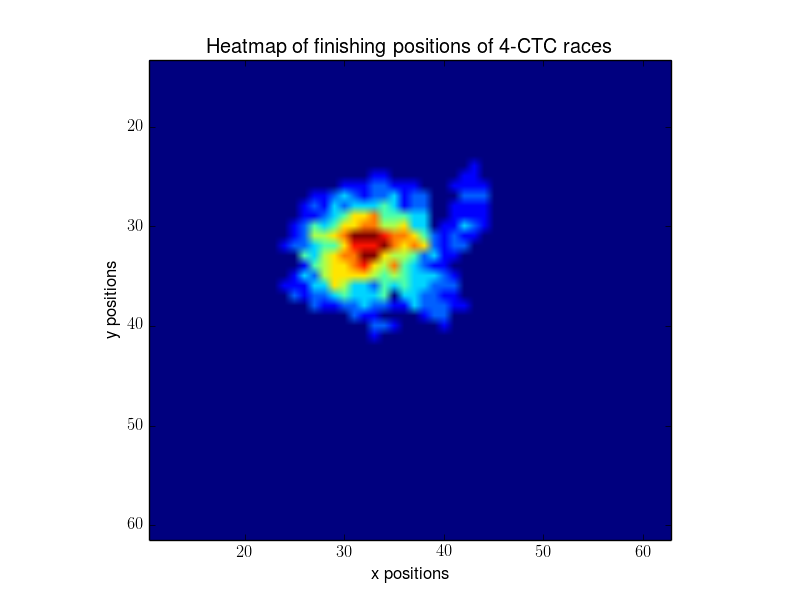
\includegraphics[scale=0.40]{img/4ctc_heat}
	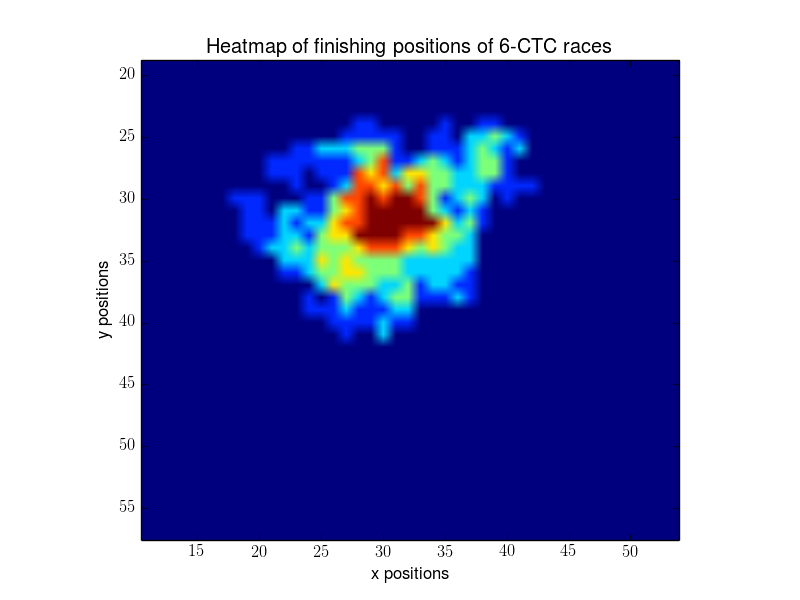
\includegraphics[scale=0.40]{img/6ctc_heat}
	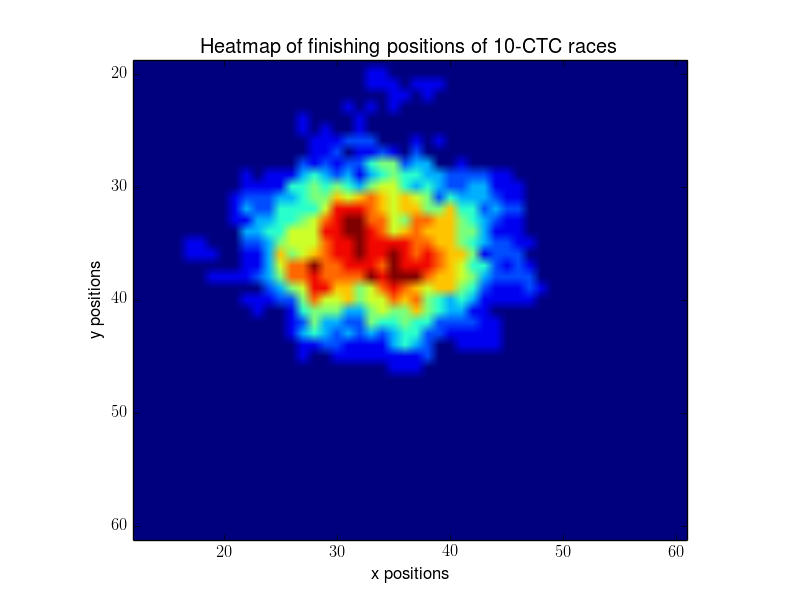
\includegraphics[scale=0.40]{img/10ctc_heat}
	\caption{Heatmaps for ending configurations of $k$-CTCs, $k\in\{1,2,3,4,6,10\}$. We can observe that $1$-CTCs and $2$-CTCs have a wider range of ending configurations while, $k=3,4,6,10$ move in more unison and have simillar ending configurations.}
	\label{heatmap}
\end{figure}

\begin{figure}[H]
	\centering
	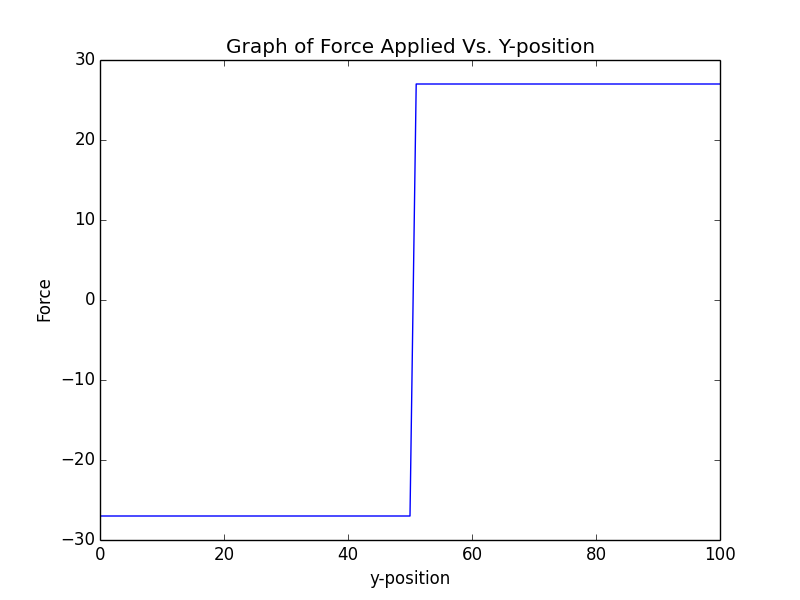
\includegraphics[scale=0.5]{img/forceapplied}
	\caption{Representation of the force applied at each y-position of the lattice. A positive force represents and acceleration in the positive y direction}
	\label{forceapplied}
\end{figure}

\begin{figure}[H]
	\centering
	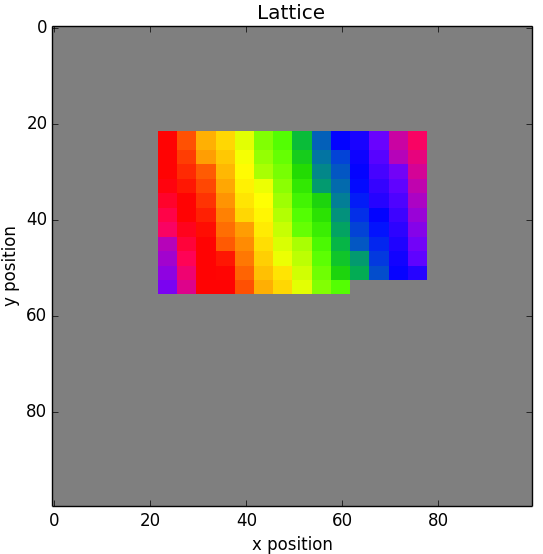
\includegraphics[scale=0.52]{img/nebula_0}
	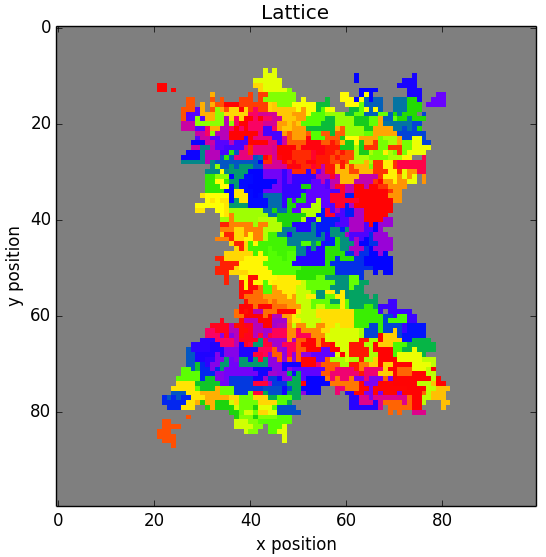
\includegraphics[scale=0.52]{img/nebula_5000}
	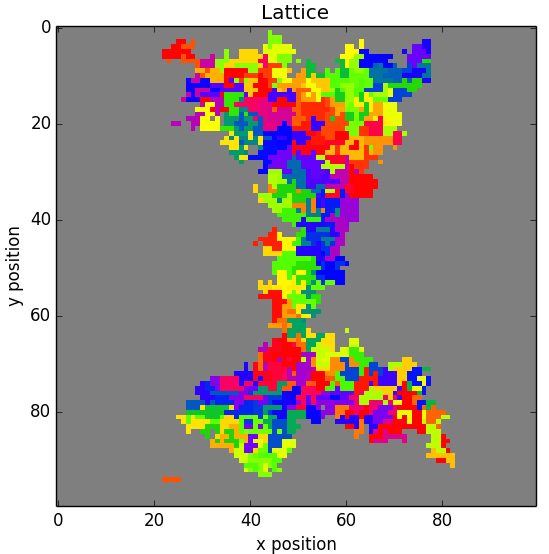
\includegraphics[scale=0.52]{img/nebula_9000}
	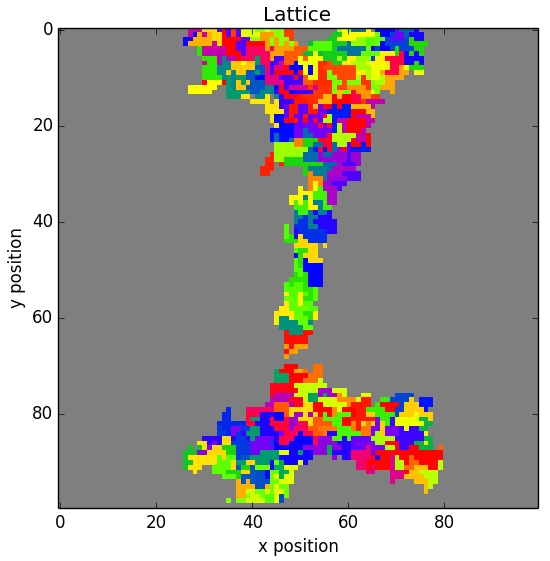
\includegraphics[scale=0.52]{img/nebula_13000}
	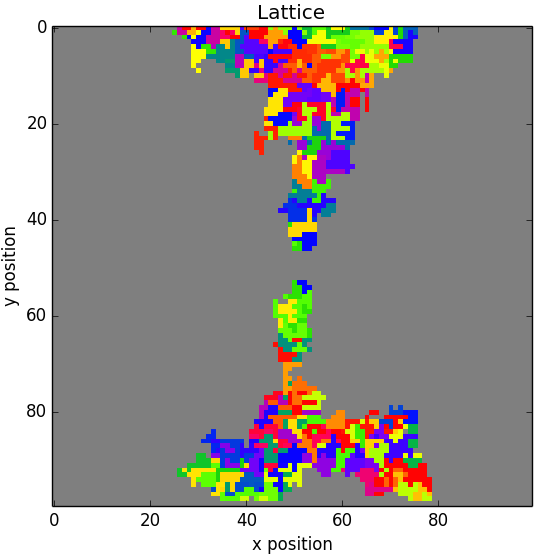
\includegraphics[scale=0.52]{img/nebula_15000}
	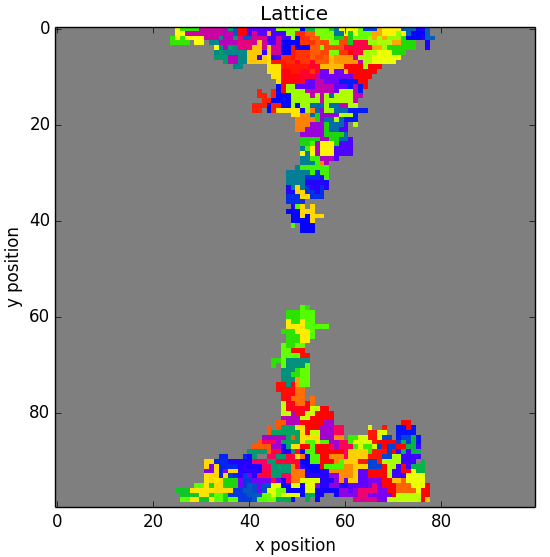
\includegraphics[scale=0.52]{img/nebula_17000}
	\caption{Time series representing the splitting of a Tissue into two by using a discontinous force. (From left to right, top to bottom: $t=0,5000,9000, 13000, 15000,17000)$}
	\label{nebula}
\end{figure}

\newpage
\bibliographystyle{abbrv}
\bibliography{396}


\end{document}